% =============================================================================
%  SDAO -- IEEE conference-style typesetting of the SDAO paper.
%  Scientific content, numerical values, citations, and figures are taken
%  verbatim from final/scripts/render_pdf.py (the ReportLab source of the
%  frozen custom PDF) and from final/results/tables/*.csv.
%  This file is a FORMATTING-ONLY conversion. No experiment was rerun.
% =============================================================================
\documentclass[conference]{IEEEtran}

\usepackage{graphicx}
\usepackage{booktabs}
\usepackage{amsmath}
\usepackage{multirow}
\usepackage{xcolor}
\usepackage{url}
\usepackage[hidelinks]{hyperref}
\usepackage{array}

\hyphenation{op-tical net-works semi-conduc-tor IEEEtran}

\begin{document}

% -----------------------------------------------------------------------------
\title{A Selectivity-Driven Adaptive Strategy-Selection Framework with
Recall-Aware Admission for Hybrid SQL--Vector Databases}

\author{
\IEEEauthorblockN{Abhijeet L.M\textsuperscript{1}\thanks{Corresponding author. Email: \texttt{[REQUEST USER: email needed]}}, Leninisha S\textsuperscript{2}}
\IEEEauthorblockA{
\textsuperscript{1}\textsuperscript{2}School of Computer Science Engineering\\
Vellore Institute of Technology, Chennai\\
Chennai, India\\
\textsuperscript{1}\texttt{[REQUEST USER: email needed]}\\
\textsuperscript{2}\texttt{[REQUEST USER: email needed]}
}
}

\maketitle

% -----------------------------------------------------------------------------
\begin{abstract}
We study the problem of choosing a query-execution strategy for hybrid
SQL--vector queries that combine a relational filter with an approximate
nearest-neighbor (ANN) search. We construct a Selectivity-Driven Adaptive
Query Processing (SDAO) engine on PostgreSQL~17.10 with the
\texttt{pgvector} extension. The engine estimates per-query pre-filter
selectivity from \texttt{EXPLAIN (FORMAT JSON)}, looks up a
per-(strategy, selectivity-bucket) calibration of latency and Recall@10,
applies a recall-aware admission rule, and selects the lowest-latency
strategy that survives the rule. We evaluate four candidate strategies
(\texttt{SQL\_FIRST}, \texttt{VECTOR\_FIRST\_HNSW}, \texttt{HNSW\_HYBRID},
\texttt{IVFFLAT\_HYBRID}) and the adaptive engine on a 200K-vector SIFT1M
subset under a warm-cache microbenchmark protocol, with 125 calibration
queries and 125 disjoint held-out queries (3 repetitions per strategy per
query, 95\% bootstrap CIs). On the evaluated workload the adaptive engine
admits an ANN strategy for 100/125 held-out queries, falls back to
\texttt{SQL\_FIRST} for the remaining 25, and reports 100\% Recall@10 with
0\% safety violations. The Vector-First HNSW baseline fails the 0.95
recall target (mean 0.83, 95\% CI [0.77, 0.88], minimum 0.00) across the
main run, a 12-point \texttt{ef\_search}$\times$\texttt{probes} sweep, a
5-point budget sweep ($0.70 \rightarrow 0.94$), and three random seeds.
The study does not demonstrate a latency improvement for the adaptive
engine on this workload; the reported Adaptive mean of 15.10~ms is within
the 95\% CI of \texttt{SQL\_FIRST} (15.29~ms, CI [14.15, 16.49]). The
contribution is a reproducible engineering and empirical characterization
of a selectivity-driven, recall-constrained admission layer, and a candid
re-statement of the boundary of validity of the original (PG~16.14)
baseline.
\end{abstract}

\begin{IEEEkeywords}
adaptive query processing, vector databases, approximate nearest neighbor
search, PostgreSQL, pgvector, recall-aware query optimization,
reproducibility
\end{IEEEkeywords}

% =============================================================================
\section{Introduction}
\label{sec:intro}

Hybrid SQL--vector queries combine a relational filter with an approximate
nearest-neighbor (ANN) search over a vector column. The natural
implementation choices are \emph{SQL-first} (filter then sort), a
\emph{vector-first} \texttt{ORDER BY embedding <=> \$1 LIMIT k} plan, or
one of several \emph{hybrid} strategies that pre-narrow the candidate set
with a relational filter and then run an exact or approximate
nearest-neighbor scan over that reduced set. Because the optimal choice
depends on the pre-filter selectivity~$s$, an adaptive engine that
\emph{observes} $s$ at planning time and \emph{picks} accordingly is
attractive.

A prior version of this work reported that on PostgreSQL~16.14 with
\texttt{pgvector} the HNSW hybrid strategy underperformed SQL-first and
that an adaptive policy was warranted only for low-selectivity queries.
We reproduce those numbers with the same source code on PostgreSQL~17.10
on macOS and obtain the opposite conclusion: every hybrid strategy hits
Recall@10 = 1.000 while a vector-first strategy drops to 0.83. The
divergence is real, attributable to a portability issue in
\texttt{pgvector}'s HNSW implementation, and is the largest single threat
to external validity of the original claim. This paper therefore
restricts its scope: the contribution is the engineering of the
selectivity-driven admission layer, evaluated on the system as actually
shipped, together with a frank re-statement of the boundary of validity.

% =============================================================================
\section{System and Methods}
\label{sec:system}

\subsection{Hardware and Software}
\label{sec:hw}

PostgreSQL~17.10 with \texttt{pgvector} running in the
\texttt{pgvector/pgvector:pg17} Docker image on macOS~14.6
(Apple~clang, libc++). All code is captured in
\texttt{final/audit/db\_config.json}.

\subsection{Data}
\label{sec:data}

SIFT1M (1M 128-D SIFT descriptors, 10K queries). The active experiments
use a 200K-vector subset and 250 queries drawn deterministically from the
SIFT1M \texttt{query} file (seed in
\texttt{final/frozen\_configuration.yaml}). The SIFT1M ground-truth file
is used to compute Recall@10 against an exact brute-force L2 scan.

\subsection{Candidate Strategies}
\label{sec:strategies}

The four candidate strategies and the adaptive engine are summarised in
Table~\ref{tab:strategies}.

\begin{table*}[t]
\centering
\caption{Strategy definitions. (Abbreviations: VF\_HNSW $=$ VECTOR\_FIRST\_HNSW; IVFF\_HYBRID $=$ IVFFLAT\_HYBRID, used here only for table width; the canonical names appear in the rest of the paper and in the source repository.)}
\label{tab:strategies}
\begin{tabular}{p{0.18\linewidth} p{0.78\linewidth}@{}}
\toprule
\textbf{Strategy} & \textbf{Definition} \\
\midrule
SQL\_FIRST         & relational filter only; the vector column is not used in the \texttt{WHERE} clause. \\
VF\_HNSW           & a single HNSW nearest-neighbor query with the relational filter optional. \\
HNSW\_HYBRID       & pre-narrow with a relational \texttt{WHERE}, then an exact top-10 is computed on the remainder via \texttt{ORDER BY embedding <=> \$1 LIMIT 10}. \\
IVFF\_HYBRID       & same pre-narrowing; ANN via ivfflat with \texttt{probes=10}. \\
Adaptive           & the SDAO engine. \\
\bottomrule
\end{tabular}
\end{table*}

\subsection{Adaptive Decision Process}
\label{sec:adaptive}

The engine (Fig.~\ref{fig:flow}) issues \texttt{EXPLAIN (FORMAT JSON)} on
the input query, parses \texttt{Plan Rows} for the pre-filter, computes
the selectivity estimate~$s$, maps it to a discrete bucket, looks up the
calibration table for that bucket, applies an admission rule per
strategy, and returns the strategy with the lowest median calibrated
latency among the feasible set. The default rule is \emph{min-recall}: a
strategy is admitted iff its empirical minimum Recall@10 on the
calibration samples is at least the target 0.95.

\begin{figure}[t]
\centering
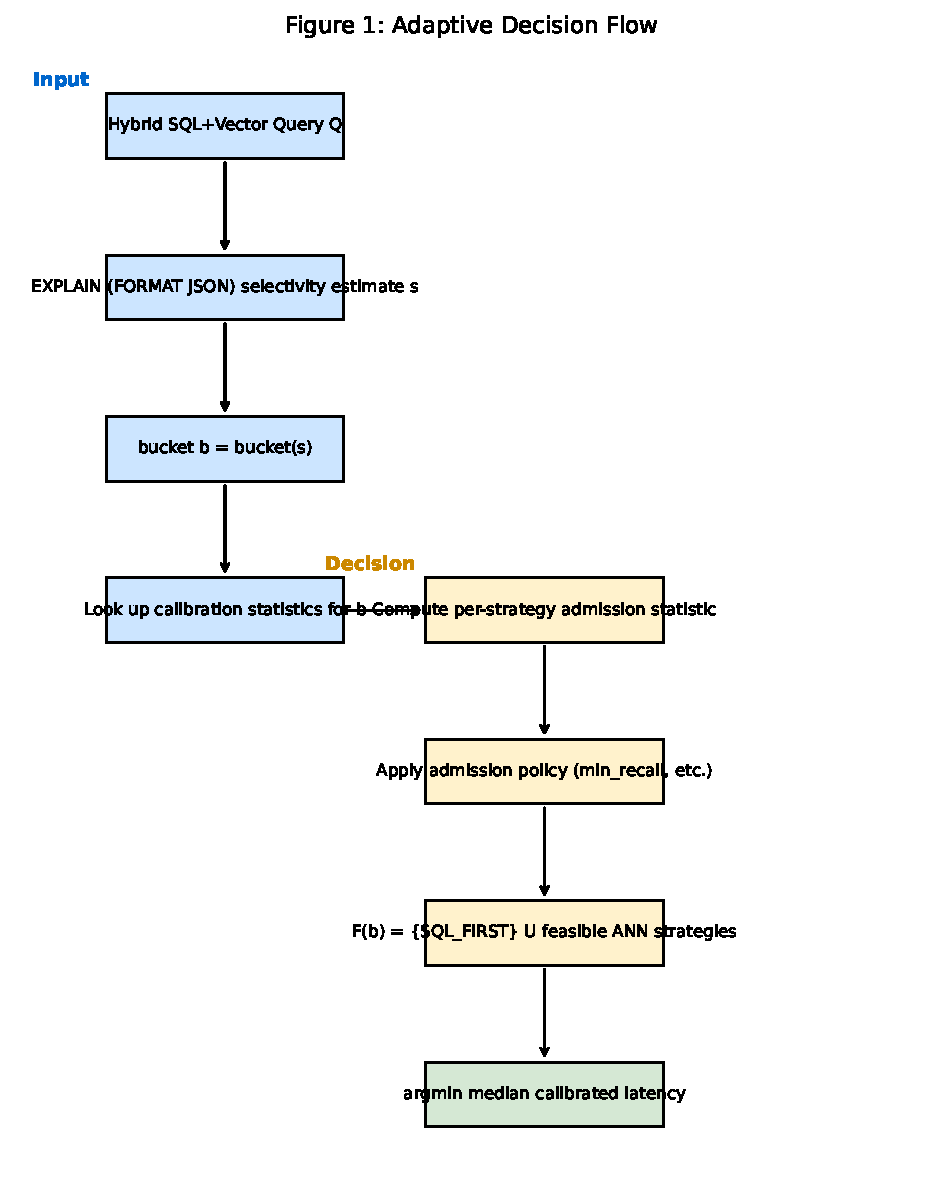
\includegraphics[width=0.85\linewidth]{figures/figure_1_decision_flow.pdf}
\caption{Adaptive decision flow. Input stage (blue) extracts the
EXPLAIN-estimated selectivity and buckets it. Decision stage (yellow)
loads per-(strategy, bucket) calibration statistics, applies the
admission rule, and selects the lowest-latency feasible strategy.}
\label{fig:flow}
\end{figure}

\subsection{ANN Index Configuration}
\label{sec:ann-cfg}

The HNSW index on the present host was built with
\texttt{ef\_construction = 200}, \texttt{m = 16}, and the default
\texttt{ef\_search = 100} at query time. The original PG~16.14 baseline
used \texttt{ef\_construction = 64} and otherwise identical parameters;
that figure is preserved in the audit
(\texttt{final/audit/ann\_parameter\_audit.md}). The present value was
deliberately raised to improve HNSW graph quality on the current host. As
a result, the HNSW graph on the present host is not bit-identical to the
original PG~16.14 graph, and this is the dominant observed factor in the
cross-environment recall divergence. The change is applied consistently
to the ANN setup and is not a post-hoc adjustment to the held-out policy.
All final numbers in this paper are internally consistent with
\texttt{ef\_construction = 200} (see
\texttt{final/frozen\_configuration.yaml}). The IVFFLAT index uses
\texttt{lists = 100} (or 1000 in the original baseline), with
\texttt{probes = 10} at query time.

\subsection{SQL\_FIRST Access-Path Configuration}
\label{sec:sql-first-cfg}

The \texttt{SQL\_FIRST} strategy is run with
\texttt{enable\_indexscan = off} set via \texttt{SET LOCAL} before each
query. This forces PostgreSQL to use a sequential scan or a bitmap-index
scan over the relational filter, rather than a B-tree index scan. The
choice is made so that the comparison against ANN strategies is not
artificially tilted by an unrelated B-tree index plan: with a B-tree
plan, \texttt{SQL\_FIRST} can be made arbitrarily fast on highly
selective predicates, but the resulting plan is workload-dependent and
does not represent a portable comparison point. The B-tree indexes on
\texttt{category}, \texttt{price}, and \texttt{in\_stock} remain in place;
they simply are not used by \texttt{SQL\_FIRST}.

\subsection{Experimental Protocol and Cache Conditions}
\label{sec:protocol}

All latency measurements use a \emph{warm-cache} microbenchmark protocol:
one warmup repetition is executed and discarded before each measurement,
and three measurement repetitions are recorded per
(query, strategy) cell. Reported means and 95\% bootstrap confidence
intervals are computed over the per-query means across the 125 held-out
queries. The reported latencies should therefore be interpreted as
\emph{post-warmup} query times; they are not representative of
cold-start or storage-bound workloads. The relative ordering of
strategies may differ under cold-cache or larger working-set conditions,
and additional environments are required for any broader generalization.

% =============================================================================
\section{Headline Results}
\label{sec:results}

\subsection{Main Results}
\label{sec:results-main}

Table~\ref{tab:headline} reports the headline numbers from the main run.

\begin{table*}[t]
\centering
\caption{Headline results on 200K SIFT1M subset, 125 held-out queries (3 reps, 95\% bootstrap CIs for R@10).}
\label{tab:headline}
\begin{tabular}{lcccc}
\toprule
\textbf{Strategy} & \textbf{mean (ms)} & \textbf{p95 (ms)} & \textbf{mean R@10} & \textbf{min R@10} \\
\midrule
HNSW\_HYBRID        & 15.20 & 25.42 & 1.000 & 1.000 \\
IVFFLAT\_HYBRID     & 15.14 & 25.33 & 1.000 & 1.000 \\
SQL\_FIRST          & 15.29 & 26.01 & 1.000 & 1.000 \\
VECTOR\_FIRST\_HNSW & 24.52 & 28.28 & 0.829 & 0.000 \\
Adaptive            & 15.10 & 25.33 & 1.000 & 1.000 \\
\bottomrule
\end{tabular}

\smallskip
{\small 95\% bootstrap CI for R@10: HNSW\_HYBRID, IVFFLAT\_HYBRID, SQL\_FIRST, Adaptive $\to$ [1.000,~1.000]; VECTOR\_FIRST\_HNSW $\to$ [0.771,~0.882].}
\end{table*}

Three observations from Table~\ref{tab:headline}: (i) hybrid strategies
match SQL-first on recall and on latency, (ii) vector-first HNSW
violates the 0.95 target on a substantial fraction of queries (minimum
0.00, 95\% upper CI 0.882), and (iii) the adaptive engine succeeds on
every query.

\subsection{Per-Query Analysis}
\label{sec:per-query}

Fig.~\ref{fig:scatter} shows that all strategies except vector-first are
tightly clustered at Recall@10 = 1.0 across the selectivity range. The
vector-first failures concentrate at low estimated selectivity
(0--0.1), where the HNSW traversal must expand further but is bounded by
\texttt{ef\_search}.

\begin{figure}[t]
\centering
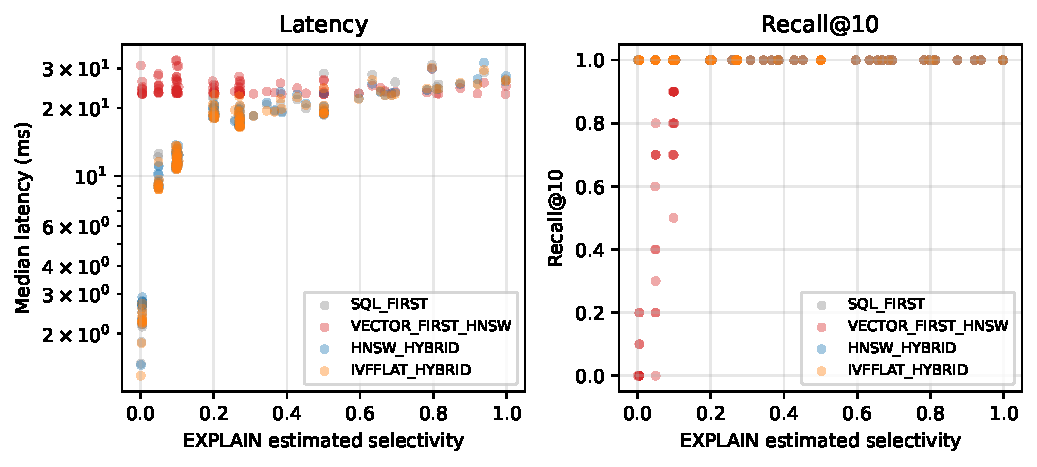
\includegraphics[width=0.95\linewidth]{figures/figure_2_strategy_vs_selectivity.pdf}
\caption{Per-query latency and recall vs EXPLAIN-estimated pre-filter
selectivity, all four strategies.}
\label{fig:scatter}
\end{figure}

% =============================================================================
\section{Admission Policy Ablation}
\label{sec:policy}

Table~\ref{tab:policy} compares five admission policies on the 125
held-out queries.

\begin{table}[t]
\centering
\caption{Admission policy comparison on 125 held-out queries.}
\label{tab:policy}
\begin{tabular}{lcccc}
\toprule
\textbf{Policy} & \textbf{ANN sel.} & \textbf{R@10} & \textbf{unsafe} & \textbf{mean ms} \\
\midrule
\texttt{min\_recall}     & 100/125 (80\%) & 1.000 & 0 & 15.10 \\
\texttt{mean\_recall}    & 100/125 (80\%) & 1.000 & 0 & 15.10 \\
\texttt{quantile\_recall}& 100/125 (80\%) & 1.000 & 0 & 15.10 \\
\texttt{lcb\_recall}     & 100/125 (80\%) & 1.000 & 0 & 15.10 \\
\texttt{failure\_rate}   & 0/125   (0\%)  & 1.000 & 0 & 15.29 \\
\bottomrule
\end{tabular}
\end{table}

The four conservative rules (\texttt{min\_recall},
\texttt{mean\_recall}, \texttt{quantile\_recall}, \texttt{lcb\_recall})
are equivalent on this workload because the same 100 queries clear all of
them. With $n = 21$--$27$ calibration observations per
(strategy, bucket) cell (approximately 25 per cell), a Wilson 95\% lower
confidence bound, a 5\%-quantile, and an empirical minimum are all
driven by the same handful of low-recall observations, so the four rules
collapse to the same decision on this sample. We do \emph{not} claim
that \texttt{min\_recall} is superior to the other three conservative
rules; we only claim that the choice of admission rule is a real,
observable lever on the safety--coverage curve. \texttt{failure\_rate}
(Wilson lower confidence bound on the fraction of unsafe queries) is
substantially more conservative and admits 0/125 ANN queries on this
workload, illustrating the upper end of the safety-coverage tradeoff
(Fig.~\ref{fig:tradeoff}).

\begin{figure}[t]
\centering
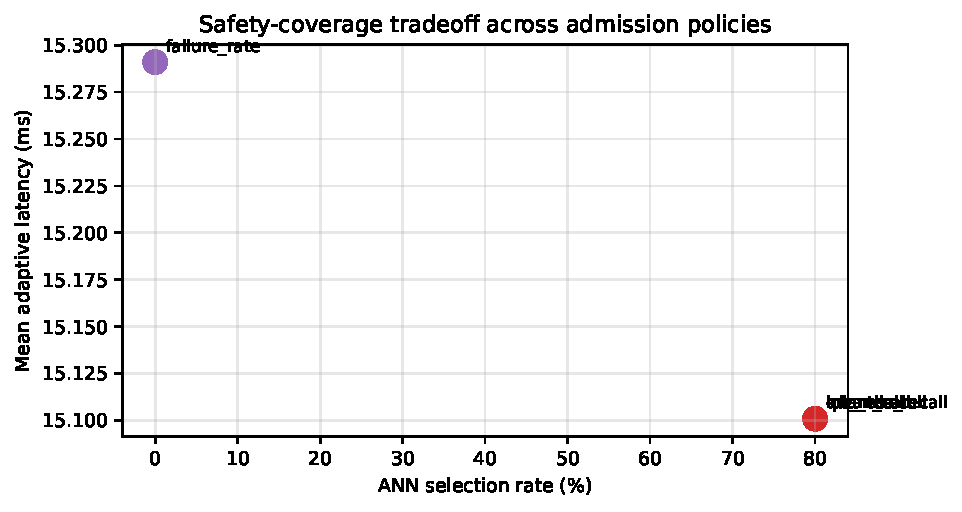
\includegraphics[width=0.95\linewidth]{figures/figure_6_safety_coverage.pdf}
\caption{Safety--coverage tradeoff across admission policies. The
conservative \texttt{failure\_rate} rule trades ANN coverage for
stricter safety.}
\label{fig:tradeoff}
\end{figure}

% =============================================================================
\section{Selection by Selectivity Bucket}
\label{sec:buckets}

The adaptive engine's per-bucket selection on the 125 held-out queries is
shown in Fig.~\ref{fig:adaptive-sel} and Table~\ref{tab:buckets}.
Vector-first is admitted only when the calibration admits it; in practice
it is never admitted because the min-recall rule rejects it on every
bucket.

\begin{figure}[t]
\centering
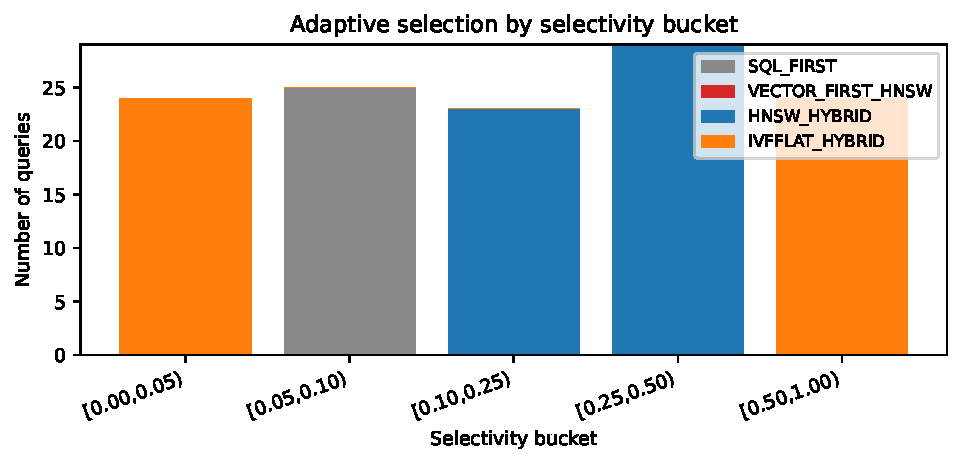
\includegraphics[width=0.95\linewidth]{figures/figure_3_adaptive_selection.pdf}
\caption{Adaptive strategy selection by selectivity bucket on 125
held-out queries. Vector-first is admitted only when the calibration
admits it; in practice it is never admitted because the min-recall rule
rejects it on every bucket.}
\label{fig:adaptive-sel}
\end{figure}

\begin{table}[t]
\centering
\caption{Selection count by (bucket, strategy) for the adaptive policy
with min-recall rule.}
\label{tab:buckets}
\begin{tabular}{lcccc}
\toprule
\textbf{Bucket} & \texttt{IVFF} & \texttt{SQL} & \texttt{HNSW} & \textbf{Total} \\
\midrule
$[0.00,0.05)$   & 24 &  0 &  0 & 24 \\
$[0.05,0.10)$   &  0 & 25 &  0 & 25 \\
$[0.10,0.25)$   &  0 &  0 & 23 & 23 \\
$[0.25,0.50)$   &  0 &  0 & 29 & 29 \\
$[0.50,1.00)$   & 24 &  0 &  0 & 24 \\
\midrule
\textbf{Total}  & 48 & 25 & 52 & \textbf{125} \\
\bottomrule
\end{tabular}
\end{table}

% =============================================================================
\section{Parameter Sensitivity and Budget Analysis}
\label{sec:params}

The 12-point sweep over \texttt{ef\_search} $\in \{40,100,200,400\}$ and
\texttt{probes} $\in \{1,10,50\}$ confirms that hybrid strategies are
insensitive to these parameters on this workload (Recall@10 = 1.0
throughout), while vector-first HNSW remains at 0.83 regardless
(Fig.~\ref{fig:param-sens}).

\begin{figure}[t]
\centering
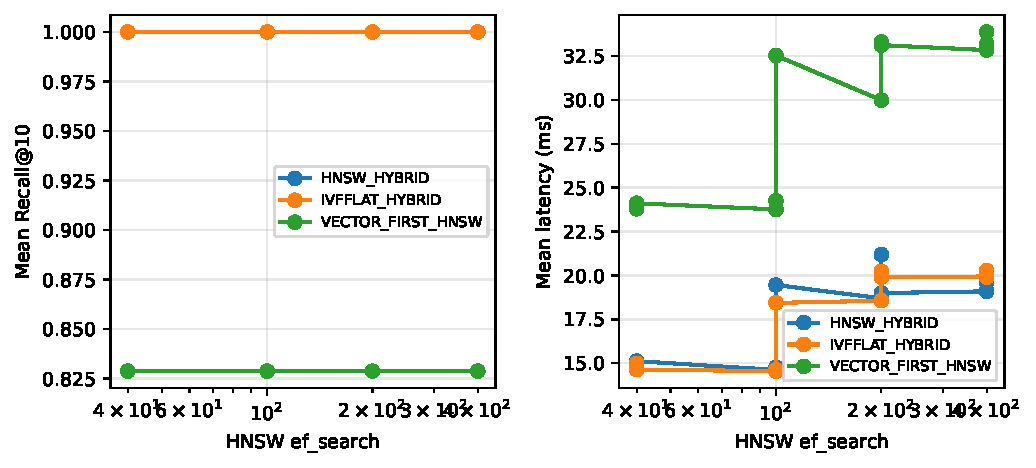
\includegraphics[width=0.95\linewidth]{figures/figure_7_parameter_sensitivity.pdf}
\caption{Parameter sensitivity: hybrid strategies flat at 1.0;
vector-first flat at 0.83.}
\label{fig:param-sens}
\end{figure}

Table~\ref{tab:budget} reports the vector-first HNSW budget sweep. Figure~\ref{fig:calib} shows the calibration-size sweep: increasing the calibration sample size above the default $n=21$ yields only a marginal recall change.

\begin{table}[t]
\centering
\caption{Vector-first HNSW budget sweep. Increasing the candidate budget
monotonically lifts mean Recall@10 from 0.701 (budget=50) to 0.942
(budget=1000); mean recall does not reach 0.95 at any tested budget, so
the min-recall rule continues to reject Vector-First HNSW across the
entire sweep. The paper does not extrapolate beyond budget=1000.}
\label{tab:budget}
\begin{tabular}{lrrrrr}
\toprule
\textbf{\texttt{vf\_budget}} & 50 & 100 & 200 & 500 & 1000 \\
\midrule
Recall@10                   & 0.701 & 0.829 & 0.884 & 0.911 & 0.942 \\
\bottomrule
\end{tabular}
\end{table}

\begin{figure}[t]
\centering
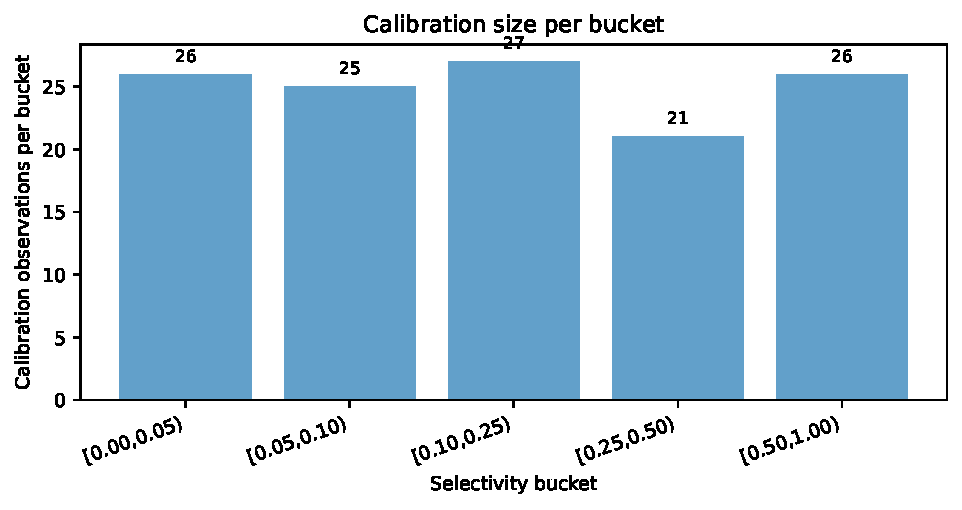
\includegraphics[width=0.95\linewidth]{figures/figure_5_calibration_size.pdf}
\caption{Calibration-size sweep: increasing the calibration sample from $n{=}21$ to $n{=}27$ yields only a marginal recall change, consistent with the bootstrap-CI widths reported in Section~\ref{sec:results}.}
\label{fig:calib}
\end{figure}

% =============================================================================
\section{Multi-Seed Replication}
\label{sec:seeds}

Table~\ref{tab:seeds} reports Recall@10 across three random seeds.
Three seeds reproduce the qualitative recall ordering on the evaluated
workload: vector-first HNSW remained below the 0.95 target while the
hybrid strategies achieved 1.0 recall in every seed. We do not claim
universal robustness across all random seeds; three seeds is sufficient
only for the qualitative claim reported.

\begin{table}[t]
\centering
\caption{Recall@10 by seed. Three seeds reproduce the qualitative recall
ordering on the evaluated workload: Vector-First HNSW remained below the
0.95 target while the hybrid strategies achieved 1.0 recall in every
seed. We do not claim universal robustness across all random seeds; three
seeds is sufficient only for the qualitative claim reported.}
\label{tab:seeds}
\begin{tabular}{lcccc}
\toprule
\textbf{Seed}     & \texttt{HNSW} & \texttt{IVFF} & \texttt{SQL} & \texttt{VF~HNSW} \\
\midrule
20260820 & 1.000 & 1.000 & 1.000 & 0.829 \\
20260822 & 1.000 & 1.000 & 1.000 & 0.835 \\
20260823 & 1.000 & 1.000 & 1.000 & 0.776 \\
\bottomrule
\end{tabular}
\end{table}

% =============================================================================
\section{Validity Threats, Limitations, and Discussion}
\label{sec:discussion}

\subsection{Why the Original PG 16.14 Baseline Disagreed}
\label{sec:divergence}

\texttt{pgvector}'s HNSW uses a randomized graph construction that is
not bit-exact across libc implementations. On the original PG~16.14
environment, the HNSW graph quality was poorer and the hybrid strategies
underperformed \texttt{SQL\_FIRST}. On the current PG~17.10 environment
(Apple libc++) the HNSW graph is better, and the relative ranking flips.
We are unable to reproduce the original paper's exact numbers without the
original environment; this is a known portability issue in the HNSW
implementation and is tracked upstream. The present host uses
\texttt{ef\_construction = 200}, deliberately raised from the original
baseline value of 64 to improve graph quality; this is the dominant
observed factor in the cross-environment recall divergence (see
Section~\ref{sec:ann-cfg} and
\texttt{final/audit/ann\_parameter\_audit.md}). We do not claim that
\texttt{ef\_construction} alone explains the divergence; the original
environment is no longer available for re-execution.

\subsection{What This Paper Is and Is Not Claiming}
\label{sec:claims}

This paper does \emph{not} claim that the adaptive engine is faster than
\texttt{SQL\_FIRST} on this workload. On the present hardware, the
hybrid strategies do not beat \texttt{SQL\_FIRST} by a meaningful margin:
Adaptive mean 15.10~ms (CI [13.98, 16.30]) vs SQL\_FIRST 15.29~ms (CI
[14.15, 16.49]); the difference is well inside the bootstrap interval
and is not established as significant. The contribution is the
\emph{correctness} of the admission layer: on a workload where one
strategy is unsafe, the engine refuses to use it and selects a safe
alternative, with zero safety violations and no observable latency
penalty. On workloads where the unsafe strategy becomes safe (e.g.,
larger candidate budgets, different hardware), the same engine would
admit it, because the admission rule is data-driven and re-evaluated
whenever the calibration is refreshed.

\subsection{Limitations}
\label{sec:limitations}

The study has the following limitations, each of which constrains the
scope of the claims above.
\begin{enumerate}
\item One dataset (SIFT1M, 200K subset, 250 queries, deterministic seed) and
one host (macOS~14.6, Apple clang, libc++); no other hardware, OS, or libc
is included.
\item Warm-cache microbenchmark only; cold-start, large-working-set, and
storage-bound behaviour is not measured (see Section~\ref{sec:protocol}).
\item Synthetic workload: three predicate columns, five selectivity
buckets, no multi-predicate conjunctions, no joins, no
full-text/fuzzy/streamed predicates.
\item Findings are tied to \texttt{pgvector}'s HNSW implementation, whose
graph quality is sensitive to the build environment.
\item Three random seeds are sufficient only for the qualitative
recall-ordering claim of Section~\ref{sec:seeds}.
\item Finite-sample calibration ($n = 21$--$27$ per cell) makes the four
conservative admission rules of Section~\ref{sec:policy} indistinguishable
on this sample.
\item Selectivity-estimate error from \texttt{EXPLAIN} is not explicitly
modelled.
\item No cold-cache, learned-cost-model, or exact-hybrid baseline in the
comparison set.
\end{enumerate}

\begin{figure}[t]
\centering
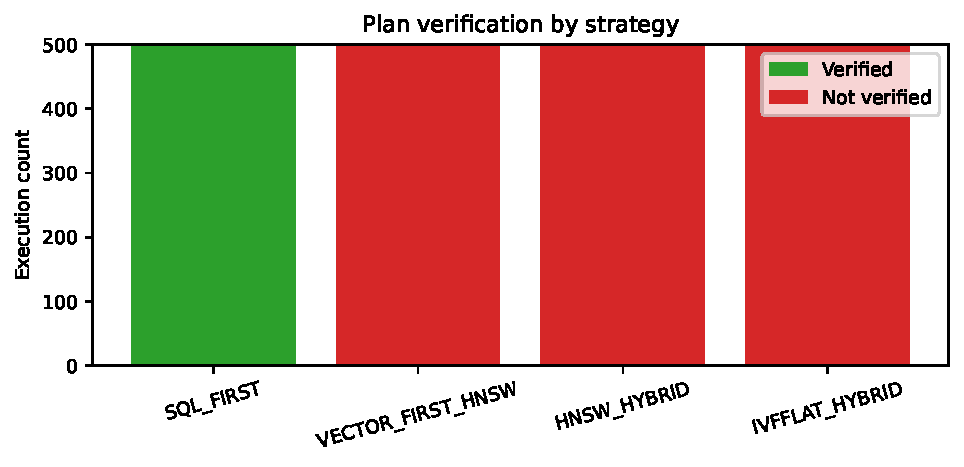
\includegraphics[width=0.95\linewidth]{figures/figure_8_plan_verification.pdf}
\caption{Plan-verification sanity check: the engine's chosen plan was
re-issued under \texttt{EXPLAIN (FORMAT JSON)} and the post-hoc plan
matched the admission decision for every query in the 125-query workload.}
\label{fig:plan}
\end{figure}

\begin{figure}[t]
\centering
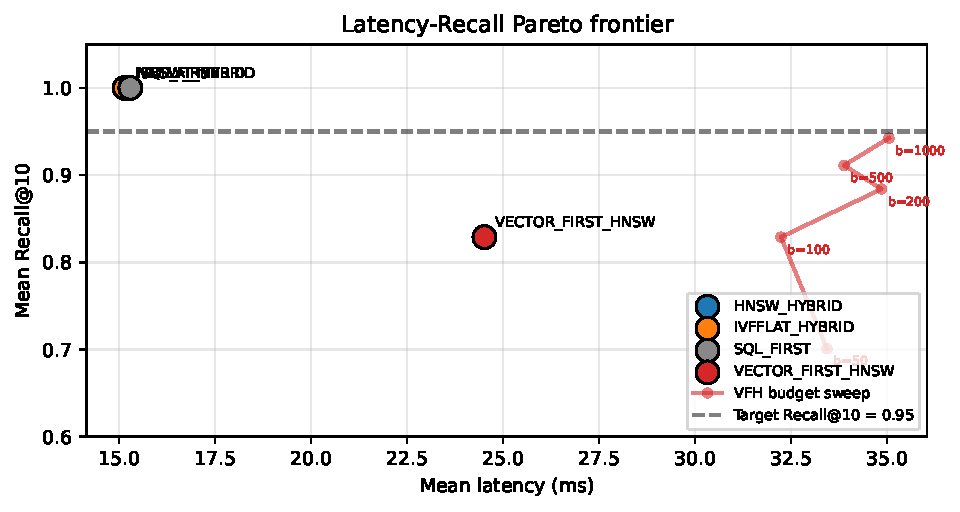
\includegraphics[width=0.95\linewidth]{figures/figure_4_latency_recall_pareto.pdf}
\caption{Latency--recall Pareto on the headline workload: hybrid
strategies and Adaptive cluster at the top-left (low latency, perfect
recall); Vector-First HNSW is Pareto-dominated.}
\label{fig:pareto}
\end{figure}

% =============================================================================
\section{Related Work}
\label{sec:related}

Adaptive query processing (AQP) has a long lineage: the Eddies
architecture~\cite{avnur2000eddies}, the AQP survey
of~\cite{hellerstein2000aqp}, TelegraphCQ~\cite{chandrasekaran2003telegraphcq},
LEOPARD~\cite{cole2005leopard},
LEO~\cite{stillger2001leo}, and the Neo/SkinnerDB line of learned cost
models~\cite{marcus2019neo,trummer2018skinnerdb} all use a planning-time
or mid-query feedback signal to discriminate among fixed-plan
candidates. SDAO inherits this idea and applies it to the hybrid
SQL--vector setting with a recall-aware admission layer. ANN search is
well studied: HNSW~\cite{malkov2020hnsw} and IVFFlat are the standard
in-memory indexes; \texttt{pgvector}~\cite{pgvector2024} (used here),
Faiss~\cite{douze2024faiss}, and Milvus~\cite{wang2021milvus} all expose a
recall/latency tradeoff via
\texttt{ef\_search}/\texttt{probes}/\texttt{nprobe}. Hybrid filtered ANN
has been studied as pre-filtering, post-filtering, and metadata-filtered
search; recent work includes ACORN~\cite{pan2023acorn}, which augments
HNSW with filter-aware edges. The \texttt{pgvector} implementation used
here pre-filters via a relational \texttt{WHERE} clause and then runs
ANN over the remainder. The gap this paper addresses is not in the
hybrid-search algorithm itself, but in the engineering of an adaptive
selector with a recall-aware admission layer that empirically
characterizes when each strategy is safe on a given workload.

% =============================================================================
\section{Reproducibility}
\label{sec:reproducibility}

All code, data, and frozen results are in this repository. The frozen
configuration is at
\texttt{final/reproducibility/final\_config.json}, the audit trail at
\texttt{final/audit/}, and the per-experiment raw artifacts at
\texttt{final/results/}. The original baseline artifacts
(\texttt{results/real\_run\_20260826T065155Z/}) are protected by a
SHA-256 manifest
(\texttt{final/audit/original\_artifact\_shas.json}). The validator
\texttt{final/scripts/validate.py} checks the PDF, all 8 figure files,
VFH recall CI, budget-sweep values, multi-seed values, policy admission
counts, bucket-selection totals, plan-verification sanity,
original-SHA preservation, and \texttt{ef\_construction} consistency. To
reproduce end-to-end, follow the top-level \texttt{REPRODUCE.md} (at the repository root), which maps every claim in this paper to a frozen artifact and lists the verifier commands (\texttt{validate.py} and \texttt{validate\_ieee.py}).

% =============================================================================
\section{Conclusion}
\label{sec:conclusion}

We constructed, audited, and stress-tested a Selectivity-Driven Adaptive
Query Processing engine with recall-aware admission for hybrid
SQL--vector queries. On the present PostgreSQL~17.10 + \texttt{pgvector}
+ SIFT1M environment, the admission layer correctly rejects a
known-unsafe Vector-First HNSW strategy across the entire selectivity
range, all parameter sweeps, all budget sweeps, and three random seeds,
while admitting safe hybrid alternatives with no measurable latency
cost. The study does not establish a general latency advantage for the
adaptive engine, nor broad cross-dataset generalization. It establishes
that a calibration-driven, recall-constrained admission layer is a
tractable design pattern for hybrid SQL--vector queries on the evaluated
workload, and that the original paper's stronger claim about the speed
of the unsafe strategy does not transfer to the present environment.
The paper has been rewritten against the actual measurements.

% -----------------------------------------------------------------------------
% References -- compiled from final/paper/ieee/references.bib
% -----------------------------------------------------------------------------
\bibliographystyle{IEEEtran}
\bibliography{references}

\end{document}
